\chapter{How to prove it?}
\begin{figure}[htp]
	\centering
	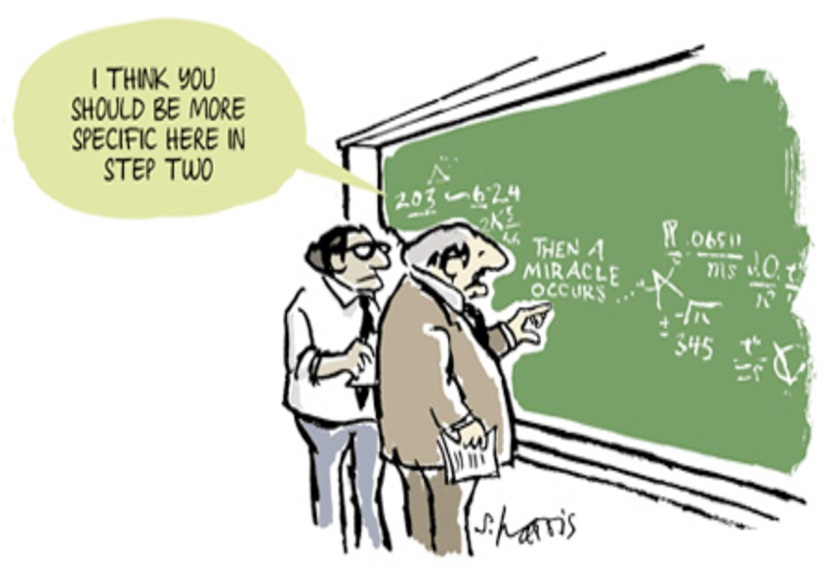
\includegraphics[width=\linewidth]{Assets/0_W-tEtGVYH9eM9HNx}
	\caption{}
	\label{fig:specific}
\end{figure}

\noindent One of the largest stumbling block in studying mathematics is learning how to prove theorems. In this post, I would share with you 3 of the most commonly used technique with at least one step by step example.
\newpage
\noindent \textbf{1. Direct proof}

\noindent Perhaps the most intuitive and straightforward way to write proofs. It goes by "\textit{If A, then B}" or  "\textit{A implies B}" or mathematically A $\Rightarrow$ B.

\noindent\textbf{Example 1} : \textit{The sum of two even numbers is also even.}
\begin{proof}
	Let $x$ and $y$ be even numbers. Since they are even, by definition they can be rewritten as $2n$ and $2m$ respectively. Thus, the sum $x+y = 2n+2m = 2(n+m)$, which is even number by definition.
\end{proof}
\noindent\textbf{Example 2} : \textit{Third Binomial Formula}
\begin{proof}
\begin{align}
(a-b)\cdot (a+b)&= a\cdot a+a\cdot b-b \cdot a-b \cdot b\\ 
			&= a^2+a \cdot b-b \cdot a-b^2\\ 
			&= a^2-b^2 
\end{align}
\end{proof}
\noindent\textbf{Example 3} : \textit{Square of odd number is also odd}
\begin{proof}
Let $x$ be odd numbers. Since it is odd, by definition it can be rewritten as $2n+1$. Thus the square product $x^2 = (2n+1)^2 = 4n^2+4n+1 = 2(2n^2+2n)+1$ which is an odd number by definition.
\end{proof}
\noindent \textbf{2. Indirect proof or proof by contradiction}

\noindent An elegant way to write a proof that might seem counter intuitive at first. It is also known as proof by contradiction and \textit{reductio ad impossibile}. It goes the following steps:
\begin{enumerate}
\item Assume the proposition to be proved is false
\item Then show that the assumption leads to mutually contradictory assertion
\item Since the assumption that the proposition is false proved contradictory, then the proposition must be true
\end{enumerate}

\noindent\textbf{Example 4} : \textit{Square root of two is irrational}
\begin{proof}
Let there be $p$ such that $p^2=2$. 
If $p$ is rational, we could write $p = \frac{m}{n}$ where $m$ and $n$ are integers that are not both even. 
This is then implies that $m^2=2n^2$ and thus $m^2$ is even. If $m^2$ is even, $m$ must be even too. Because $m$ is even, $m^2$ is divisible by 4 which in turn implies that $n^2$ is even and therefore $n$ is even.
This contradicts with our earlier assumption that $m$ and $n$ are integers that are not both even and therefore, a rational $p$ could not exist.
\end{proof}

\noindent\textbf{Example 5} : \textit{There exist no integers a and b for which 6a + 3b = 1}
\begin{proof}
Let us first assume that such $a$ and $b$ exist.
Dividing by 3 gives us: $2a+b=\frac{1}{3}$
which is a contradiction since $2a+b$ is an integer but $\frac{1}{3}$ is not. Therefore there exist no such integers a and b
\end{proof}

\noindent \textbf{3. Mathematical Induction}

\noindent Mathematical induction is usually taught together with series and sequences. It is a powerful tool to prove series and sequences. It is split into two steps:
\begin{enumerate}
\item Initial case : prove that the statement holds for 0 and or 1
\item Induction step: prove that the statement holds for every $n$, if it holds for every $n$, then it also holds for $n+1$
\end{enumerate}

\noindent\textbf{Example 6} : \textit{Little Gauss (Arithmetic progression)}
\begin{equation}
\sum_{i=1}^n i= \frac{n\cdot(n+1)}{2}
\end{equation}
\begin{proof}
\begin{align}
(a-b)\cdot (a+b)&= a\cdot a+a\cdot b-b \cdot a-b \cdot b\\ 
			&= a^2+a \cdot b-b \cdot a-b^2\\ 
			&= a^2-b^2 
\end{align}
\end{proof}
\noindent\textbf{Example 7} : \textit{Bernoulli's inequality}
\begin{equation}
(1+x)^n \ge 1+nx
\end{equation}
